
\subsection{Projector}
The projector serves as a component in the sub-network component of siamese networks.
Its main function is to transform a lower-dimensional encoded representation into a higher dimensional space suited for a SSL loss function. Common SSL techniques using projectors 
include BYOL, SimCLR and Barlow Twins.


\subsubsection{Projector architecture}
The projector architecture is designed with the objective of expanding the number of features through fully connected layers. The arcitecture used in this methology consist of the following components.
\todo{Bit vague}
\begin{itemize}
    \item \textbf{Global max pooling.} Condenses the input encodings into a condensed and robust set of features. This helps distill the most salient aspects of the encoded data.
    \item \textbf{Fully connected layers}. Broadens the dimensions and learns weights and biases that emphasize differences 
    \item \textbf{batch normalization}
    \item \textbf{ReLu activation function}
\end{itemize}


\section{Additional Machine Learning Algorithms}
\subsection{Support Vector Machines, SVM}
Support Vector Machines (SVM) is a supervised machine learning algorithm widely used for classification and regression tasks. The core idea of SVM is to establish an optimal hyperplane that maximizes the margin between different class labels. This approach is effective in high-dimensional spaces, addressingthe curse of dimensionality through its dependence on support vectors.
These support vectors are a critical subset of the training data that influences the construction of the decision boundary. SVM's adaptability is further enhanced by its capability to incorparate various kernel functions, such as linear and radial basis functions, to suit different types
of data distributions. The foundation of SVM is largely based on the work done by Vapnik et al\cite{svm}.
\begin{figure}[H]
    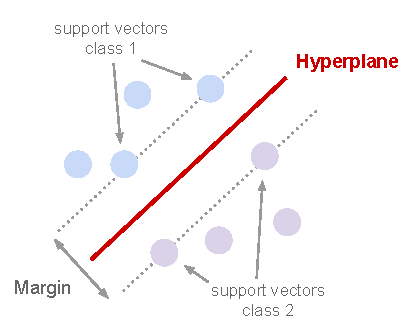
\includegraphics[scale=0.8]{figures/figure-pdf/SVM.pdf}
    \caption{Vizualisation of the hyperplane, margin and support vectors in a SVM procedure.}
\end{figure}


\subsection{K-Neares Neighbors, KNN}
K-Nearest Neighbors (KNN) is a versatile supervised learning algorithm that classifies data points based on the majority class of their K nearest neighbors.
It operates under the assumption that similar data points are likely to be close in proximity. One of the key strengths of KNN is its simplicity and effectiveness in classification tasks. 
However the KNNs performance is significally impacted by the choice of K and the distance metric used, visualized in fig \ref{fig:knn}.
The choice of K is often determined by techniques like cross validation.

\begin{figure}[H]
    \centering
    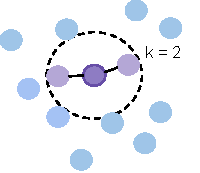
\includegraphics[width=0.3\textwidth]{figures/figure-pdf/2NN.pdf}
    \hspace{1cm}
    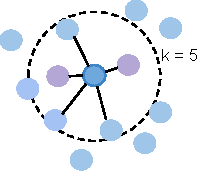
\includegraphics[width=0.3\textwidth]{figures/figure-pdf/5NN.pdf}
    \caption{Classification of middle point in a KNN procedure. For $k=2$ the majority vote is purple while for $k=5$ it is blue.}
    \label{fig:knn}
\end{figure}

\subsection{KMeans and Silhouette Score}
K-Means is a popular unsupervised learning algorithm used primarely for clustering.
Its goal is to partition the data into K distinct clusters, each represented by its centroid, which is the mean of the points in the cluster.
The algorithm iteratively assigns each data to the neares cluster, based on the Euclidian distance to the centroid, and then recalculates the centroids. 
This process repeats until the centroids stabilize or a certain iteration criteria is met. 

The Silhouette Score is a metric for evaluating the effectiveness of the clustering process. It measures how similar an object is to its own cluster (cohesion) compared to other clusters (separation).
The score ranges from -1 to 1, where a high value indicates that the object is well matched to its own cluster and poorly matched to neighboring clusters.

\begin{itemize}
    \item \textbf{Cohersion (a)}. It measures the average distance of the data point from all other points in the same cluster. \\
    \item \textbf{Seperation (b)}. It is the average distance of the data point to the points in the nearest cluster that the data point is not apart of.
\end{itemize}

The formula for the Silhouette score of a single data point ($i$) is given by:
\begin{equation}
    S_i = \frac{b_i-a_i}{\text{max}(a_i, b_i)}
\end{equation}

The overall silhouette score, $S$, for a dataset is the mean of the silhouette score of each data point.
\begin{figure}[H]
    \centering
    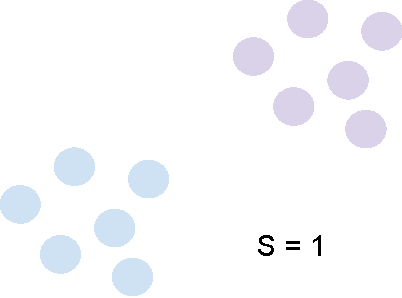
\includegraphics[width=0.3\textwidth]{figures/figure-pdf/Shigh.pdf}
    \hspace{1cm}
    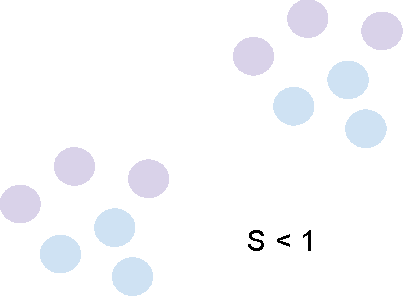
\includegraphics[width=0.3\textwidth]{figures/figure-pdf/Slow.pdf}
    \caption{Illustration of the silhuette score metric applied. On the left we see well seperated clusters with a silhouette score equal to 1. On the right a not so well seperation, giving a silhouette score less than 1.}
    \label{fig:knn}
\end{figure}

